\documentclass[tikz]{standalone}

\usetikzlibrary{arrows.meta}
\tikzset{>=stealth}

\begin{document}
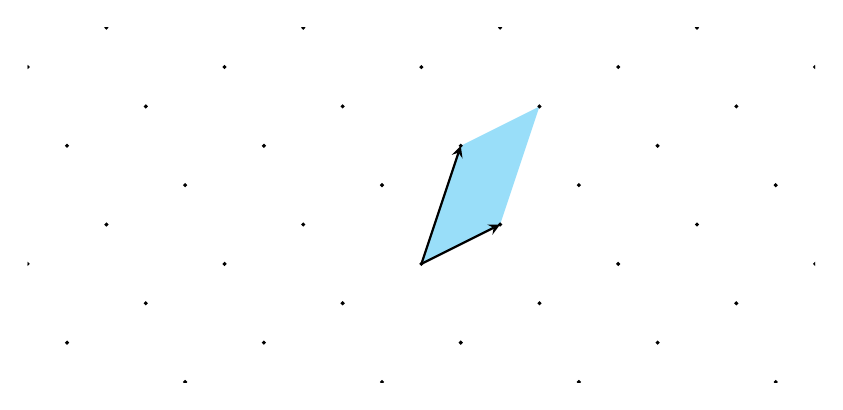
\begin{tikzpicture}[scale=0.5]
  \clip (-10, -3) rectangle (10, 6);
  \fill[color=cyan!40]
    (0, 0) -- (2, 1) -- ++(1, 3) -- (1, 3);
  \draw[->, thick] (0, 0) -- (2, 1);
  \draw[->, thick] (0, 0) -- (1, 3);

  \foreach \x in {-10,...,10}
  \foreach \y in {-10,...,10}
    \draw[fill] (2*\x + \y, \x + 3*\y) circle (1pt);
\end{tikzpicture}
\end{document}
